\subsection{MDP-Tetris}

When running the experiments, the source code of the MDP-Tetris
\citep{mdptetris} was used to emulate the Tetris games.
The source code is accompanied with files that describe the
various existing features. These files contains the identifiers of 
each feature to use, as well as two numbers respectively describing 
the agents reward function and how to evaluate a game over state. 
The number for the reward function has remained unchanged at $0$ 
during all experiments. The "game-over" evaluation was for the
Bertsekas feature set initially set to $0$. Setting the 
"game-over" evaluation to $0$ means that the agent will not 
distinguish between regular moves and moves that results in losing
the game. When running the experiments with this setting, a large portion
of the agents never exceeded a zero mean score. However, setting the value
to $-1$, meaning that a "game-over" move yields $-\infty$ reward, 
none of the experiments got stuck on only zero scores. An example
of the layout of the feature file can be seen in figure \ref{fig:featfile}.
\begin{figure}[h!]
\centering
\begin{lstlisting}
0    <- Describes the reward function
-1   <- Actions leading to game over is avoided at all cost
22   <- The policy contains 22 features
8 0  <- The feature with id 8 initially has weight 0
...  <- The remaining 21 features
\end{lstlisting}
\caption{Example of a file that describes a feature set. \label{fig:featfile}}
\end{figure}

\subsubsection{Game complexity \label{HardTetris}}
In order to reduce the runtime of experiments, to allow us more experiments in the evaluations, we can increase the "difficulty" of Tetris, by adjusting either the board size and/or adjusting the frequency of certain pieces. This has also been described before by Amine Boumaza, \citep{boumaza2009}.\\
To increase the difficulty of the game,
in our "Hard" Tetris, the s-block and z-block appear twice as often 
as the other pieces.

\begin{figure}[H]
\begin{center}
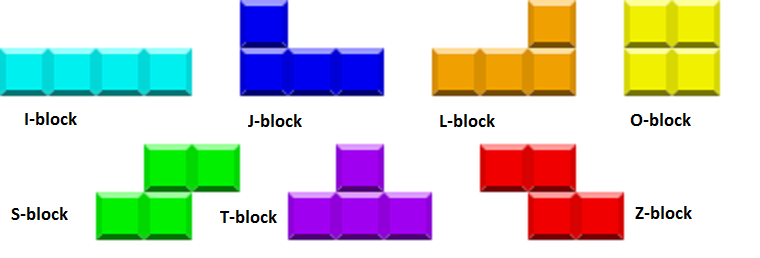
\includegraphics[scale=0.6]{img/Pieces}
\end{center}
\caption{Regular Tetris pieces \label{fig:TetrisPieces}}
\end{figure}

We want to test whether the game complexity has an impact on the performance of the algorithms,
therefore we want to test the two algorithms with Bertsekas/Tsitsiklis featureset, using Normal Tetris and Hard Tetris.\\

\textbf{Results}\\
In the following figure is depicted the mean results of 30 individual experiments using Cross Entropy and CMA, applied to both Hard Tetris and Normal Tetris. The general settings of the experiments can be seen in the appendix section, \ref{AppendixGameComplexity}.

\begin{table}[H]
\centering
\small
\begin{tabular}{c c c r r r r}
Tetris Type & Optimizer & mean & Q1 & Q2 & Q3\\
\hline
Hard & Cross Entropy & $1633.607$ & $1357.170$ & $1606.565$ & $1938.71$\\
Normal & Cross Entropy & $100059.463$ & $79357.440$ & $105999.500$ & $111047.500$\\
Hard & CMA & $449.352$ & $201.850$ & $300.300$ & $529.350$\\
Normal & CMA & $49760.161$ & $42528.740$ & $49915.700$ & $67764.729$\\
\end{tabular}
\caption{Experiment testing game Normal Tetris against Hard Tetris}
\end{table}

\begin{figure}[H]
\centering
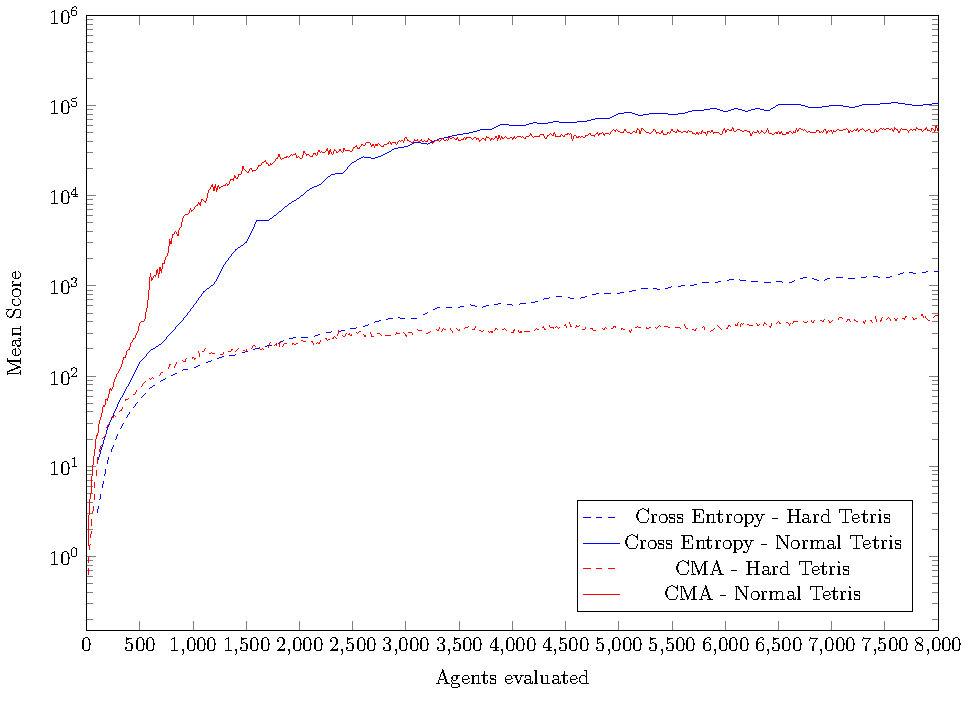
\includegraphics[scale=1]{data/complexity/mean/PlotFile.pdf}
\caption{Experiment testing Normal Tetris against Hard Tetris}
\end{figure}

\textbf{Analysis and discussion}\\
The results indicate that using Hard Tetris does not impact the general development of the algorithms, meaning we are able to use the harder Tetris for further experiments. From the graph it appears that the harder Tetris simply shifts the score compared to normal Tetris.
\\


\subsubsection{Comparison of featuresets  \label{compoffeatureset}}
As described in section \ref{ConfigureTetrisBackground}, there are different kind of featuresets which
impacts the performance of the agents. In our upcoming experiments, we are going to
use both the Dellacherie and Bertsekas/Tsitsiklis featureset. For our initial comparison experiments
we are going to use the Bertsekas/Tsitsiklis featureset, since other researchers report
a lower score with the Bertsekas/Tsitsiklis featureset compared with the Dellacherie featureset
\citep{thiery:09}. Compared to the \citep{thiery:09} experiments, we don't want to maximize the
final score, but rather maximize the score with the lowest possible number of 
games evaluated.\\
It's important to note that we are not going to conduct comparison experiments with different
featuresets in the same experiment, since the algorithms needs to be on equal terms.\\
\\
We want to test whether the featureset has an impact on the performance of the algorithms,
therefore we want to test the two algorithms with both the Dellacherie and Bertsekas/Tsitsiklis featureset.\\
From the game complexity section \ref{HardTetris}, we have verified that using Hard Tetris
\citep{boumaza2009} does not have an impact on the development of the two algorithms.
Therefore, to prevent long runtimes, the games were simulated
using Hard Tetris.\\

\textbf{Results}

In the following figures the mean results of 30 runs of both CMA and Cross 
Entropy is presented. The settings for Cross Entropy remains at constant noise
with a noise term of $z_t = 4$ and an initial sigma of $\sigma_0 = 100.$, 
and the CMA with $\sigma_0 = 1$.\\
\\
Figure \ref{fig:featuresetCompareBertsekas} shows the experiment with the 
Bertsekas featureset. This shows that when running the algorithms with a
harder game, the algorithms behave mostly the same as with regular 
Tetris. Namely that CMA converges faster than Cross Entropy, 
but is eventually outperformed.

\begin{figure}[H]
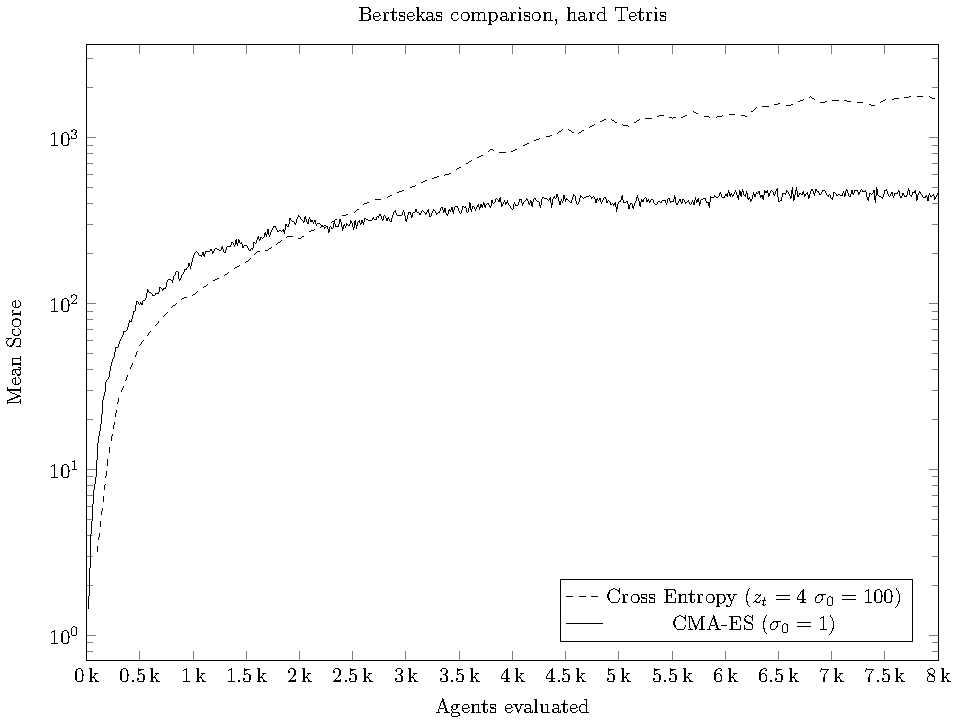
\includegraphics[scale=1]{plots/plotBertsekasCmaVsCEHardTetris}
\caption{Comparison between CMA-ES and Cross Entropy 
using hard Tetris and the Bertsekas featureset 
\label{fig:featuresetCompareBertsekas}}
\end{figure}

When using the Dellacherie featureset a similar behaviour is observed.
However, the convergence seems to occur earlier and with a higher score
(figure \ref{fig:featuresetCompareDellacherie}).

\begin{figure}[H]
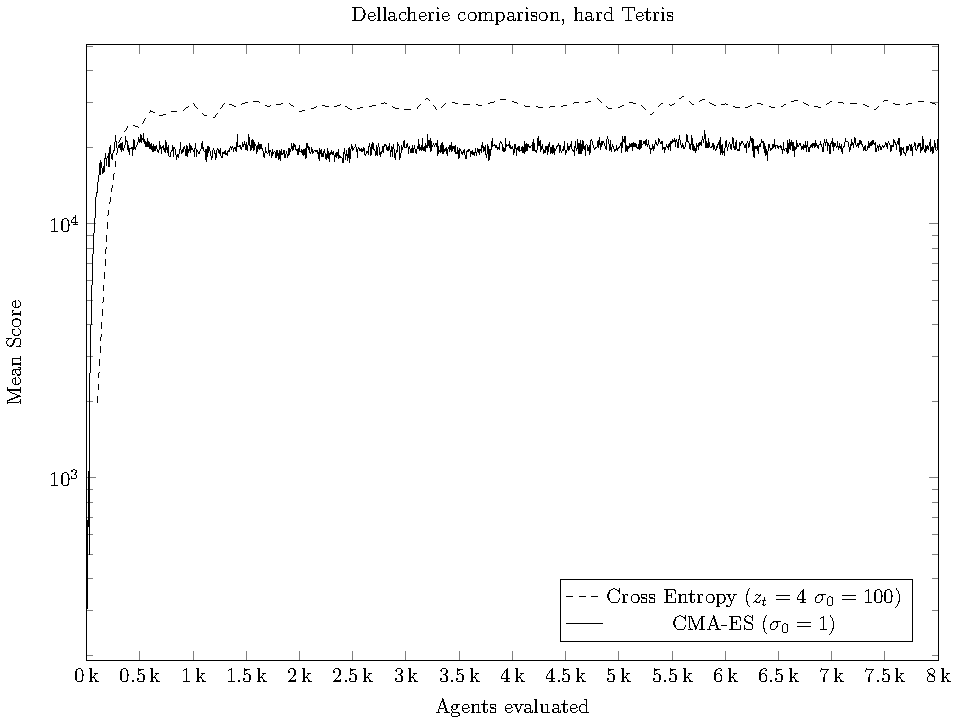
\includegraphics[scale=1]{plots/plotDellCmaVsCEHardTetris}
\caption{Comparison between CMA-ES and Cross Entropy 
using hard Tetris and the Dellacherie featureset
\label{fig:featuresetCompareDellacherie}}
\end{figure}

\textbf{Analysis and discussion}

The experiment with different featuresets indicates that the behaviour 
is not heavily dependant on the featureset.
It appears that changing the featureset simple shifts the score, but does not affect the development of the graphs.\\
Therefore, we conclude that changing the featureset does not invalidate
the comparison of the two optimization algorithms.

